\subsection{默认字节序转换与RISC-V B拓展rev8转换}
查看开发板CPU所支持的指令集如下图:
\begin{figure}[H]
    \centering
    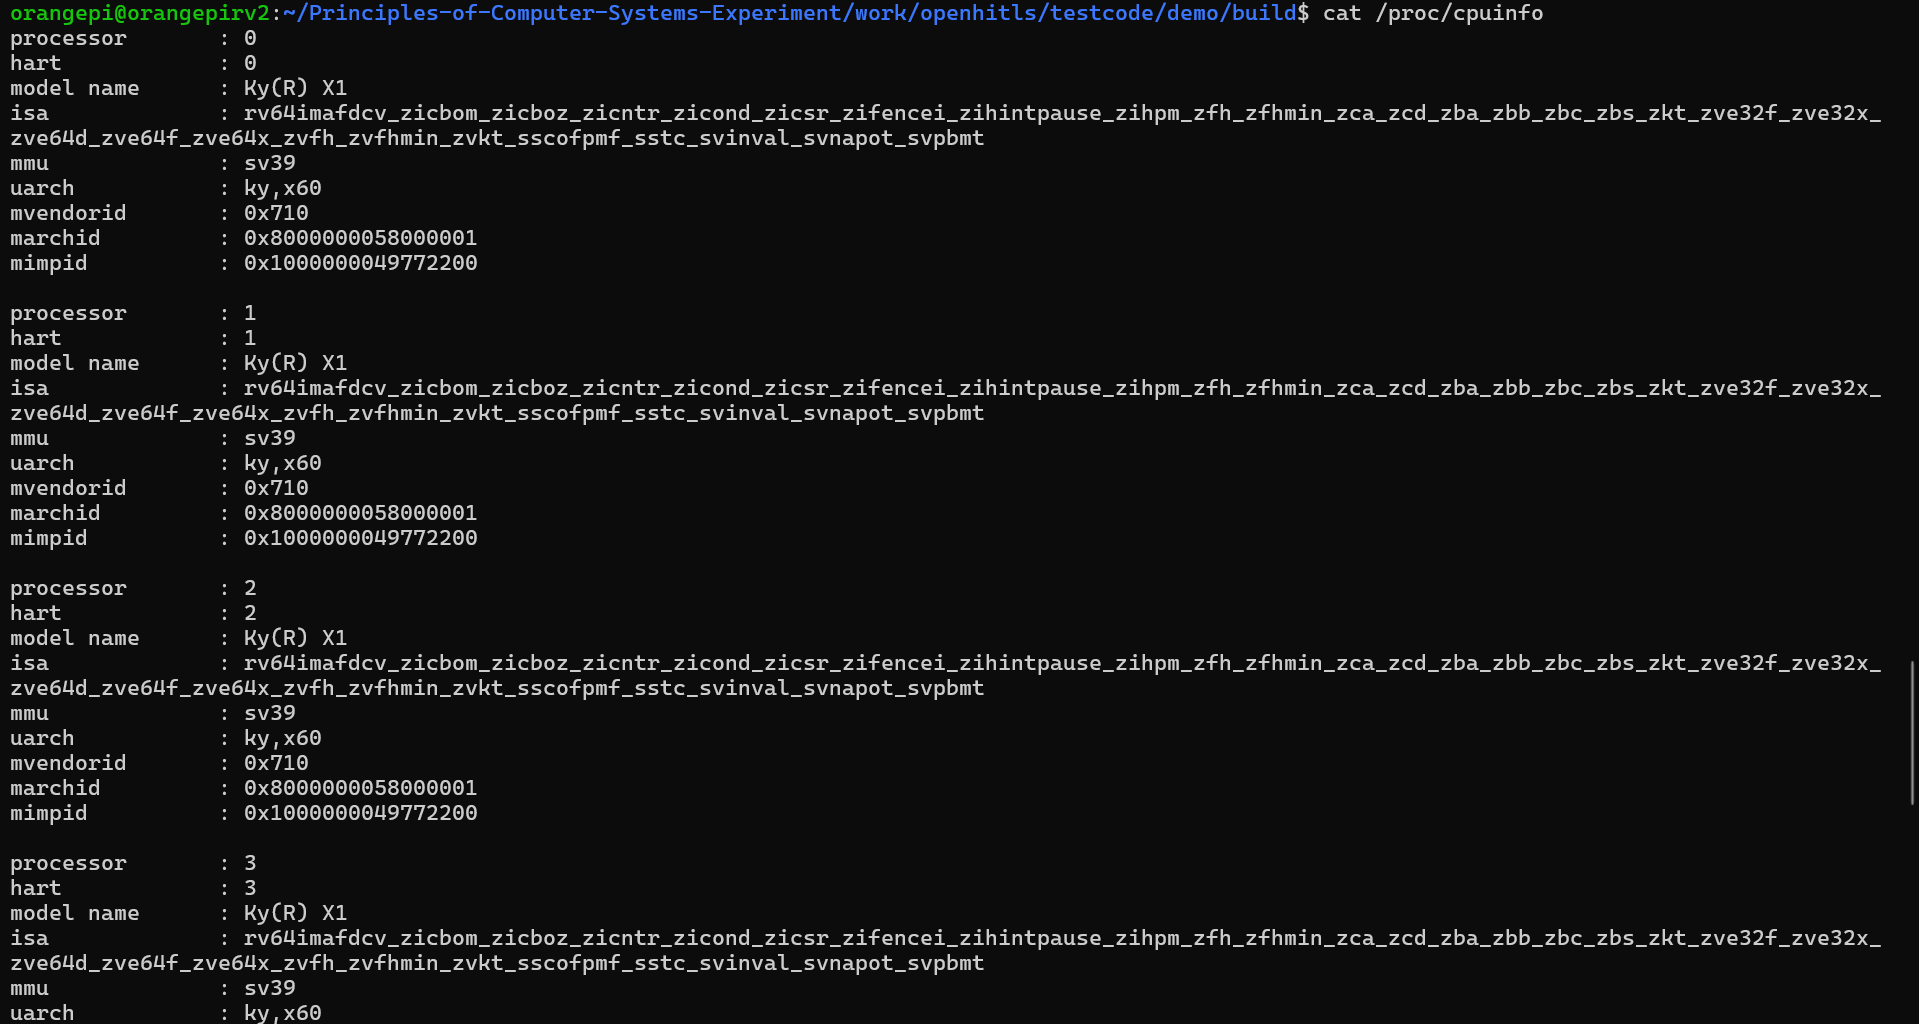
\includegraphics[width = 1\textwidth]{figure/CPU_instruction_set.png}
    \caption{开发板CPU信息}
\end{figure}
可以看到该板支持zbb,因此可以在编译时启用该拓展。该拓展的优化原理在于:
\begin{itemize}
    \item 对字节序转换的优化:标准SM4中对串\texttt{01234567}的解释为:
\[  01\ 23\ 45\ 67  \]
即大端序,而在RISC-V中却是小端序,因此sm4LoadBlock()函数需要转换。普通实现时的代码
\begin{ccode}
x =
(in[0]<<24)
|
(in[1]<<16)
|
(in[2]<<8)
|
in[3];
\end{ccode}
对应的汇编代码为:
\begin{asmcode}
lbu
slli

lbu
slli

lbu
slli

or
or
or  
\end{asmcode}
需要很多条指令才能完成,而使用Zbb拓展中的rev8指令则可直接完成这一功能,即直接
\begin{asmcode}
lw
rev8
\end{asmcode}
即可完成,使得如sm4LoadBlock()、sm4StoreBlock()函数得到加速。
\item Zbb对L变换的优化:
针\texttt{ROL(x,10)}操作,编译器默认生成:
\begin{asmcode}
slli t1,x,10
srli t2,x,22
or   t1,t1,t2
\end{asmcode}
即:
\[  (x << 10)| (x >> 22)   \]
这需要2次shift和1次or共3条指令,对于SM4每轮的四次ROL则总共需要12条指令。Zbb拓展提供rori(Rotate Right Immediate)指令,
可直接实现一次ROL操作,因此每轮L变换仅需4条指令即可完成。
\end{itemize}
对比代码不同编译方式运行结果如下:
\begin{figure}[H]
\centering
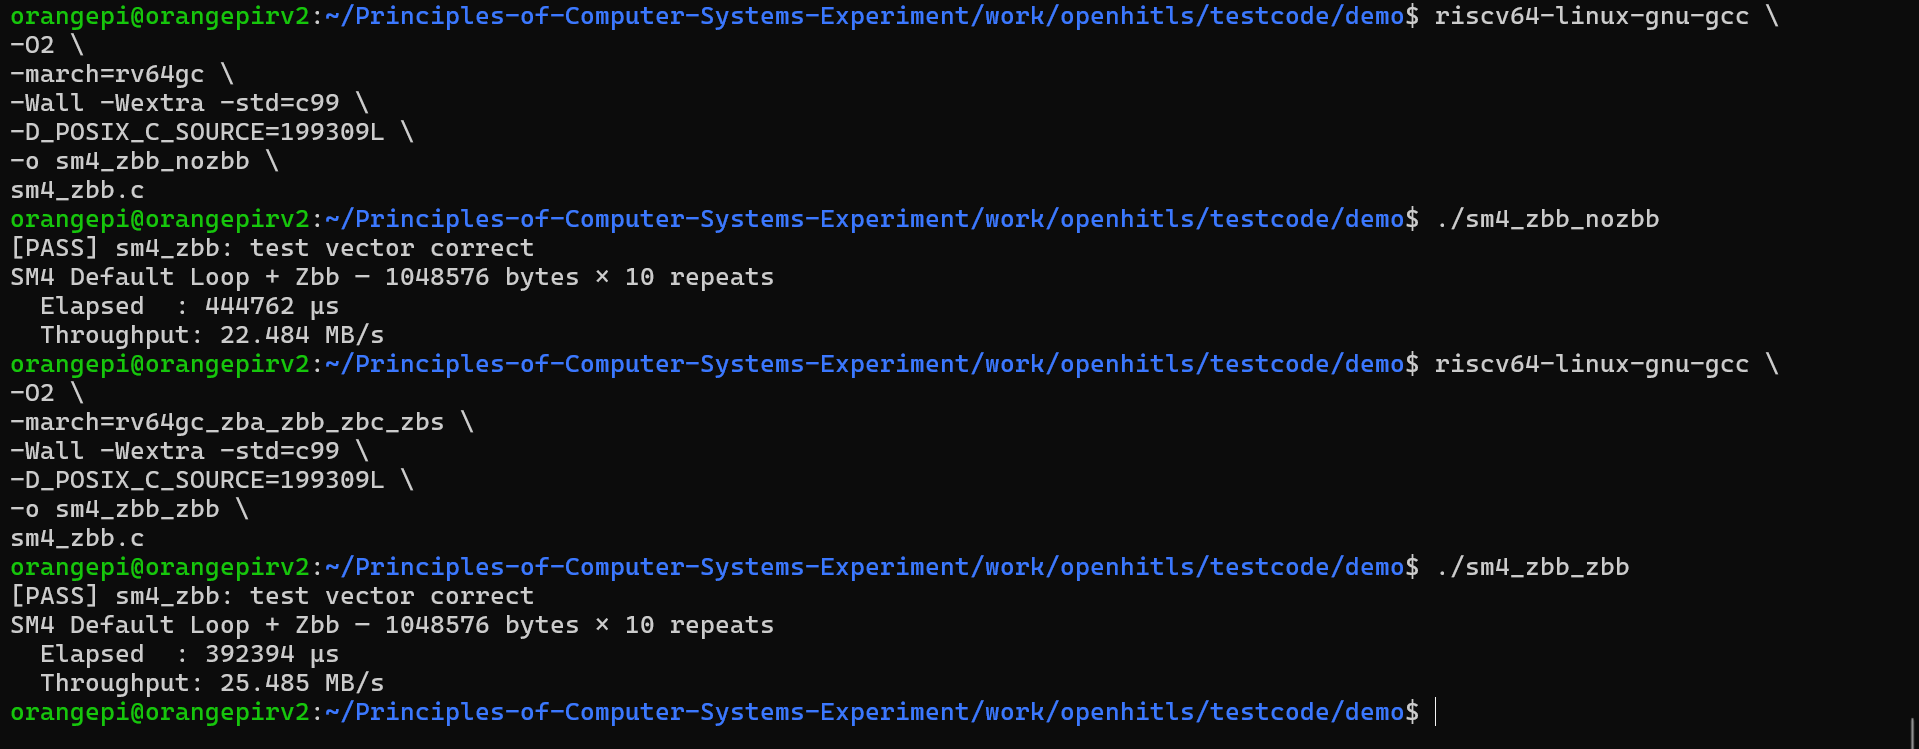
\includegraphics[width = 1\textwidth]{figure/sm4_zbb.png}
\caption{SM4默认字节序转换与rev8转换}
\end{figure}
可以看到拓展指令能小幅提升程序效率与吞吐量。
